%source: AUT-CE-LC HW10-Q3


مدار شکل زیر را درنظر بگیرید.

\begin{enumerate}
	\item 
	جدول مشخصه آن را رسم کنید و معادلات مشخصه را برای هریک از خروجی‌های مدار به‌دست آورید.
	
	\item 
	دیاگرام حالت\footnote{\lr{State Diagram}} آن را رسم کنید.

\end{enumerate}


\begin{figure}[h]
	\centering
	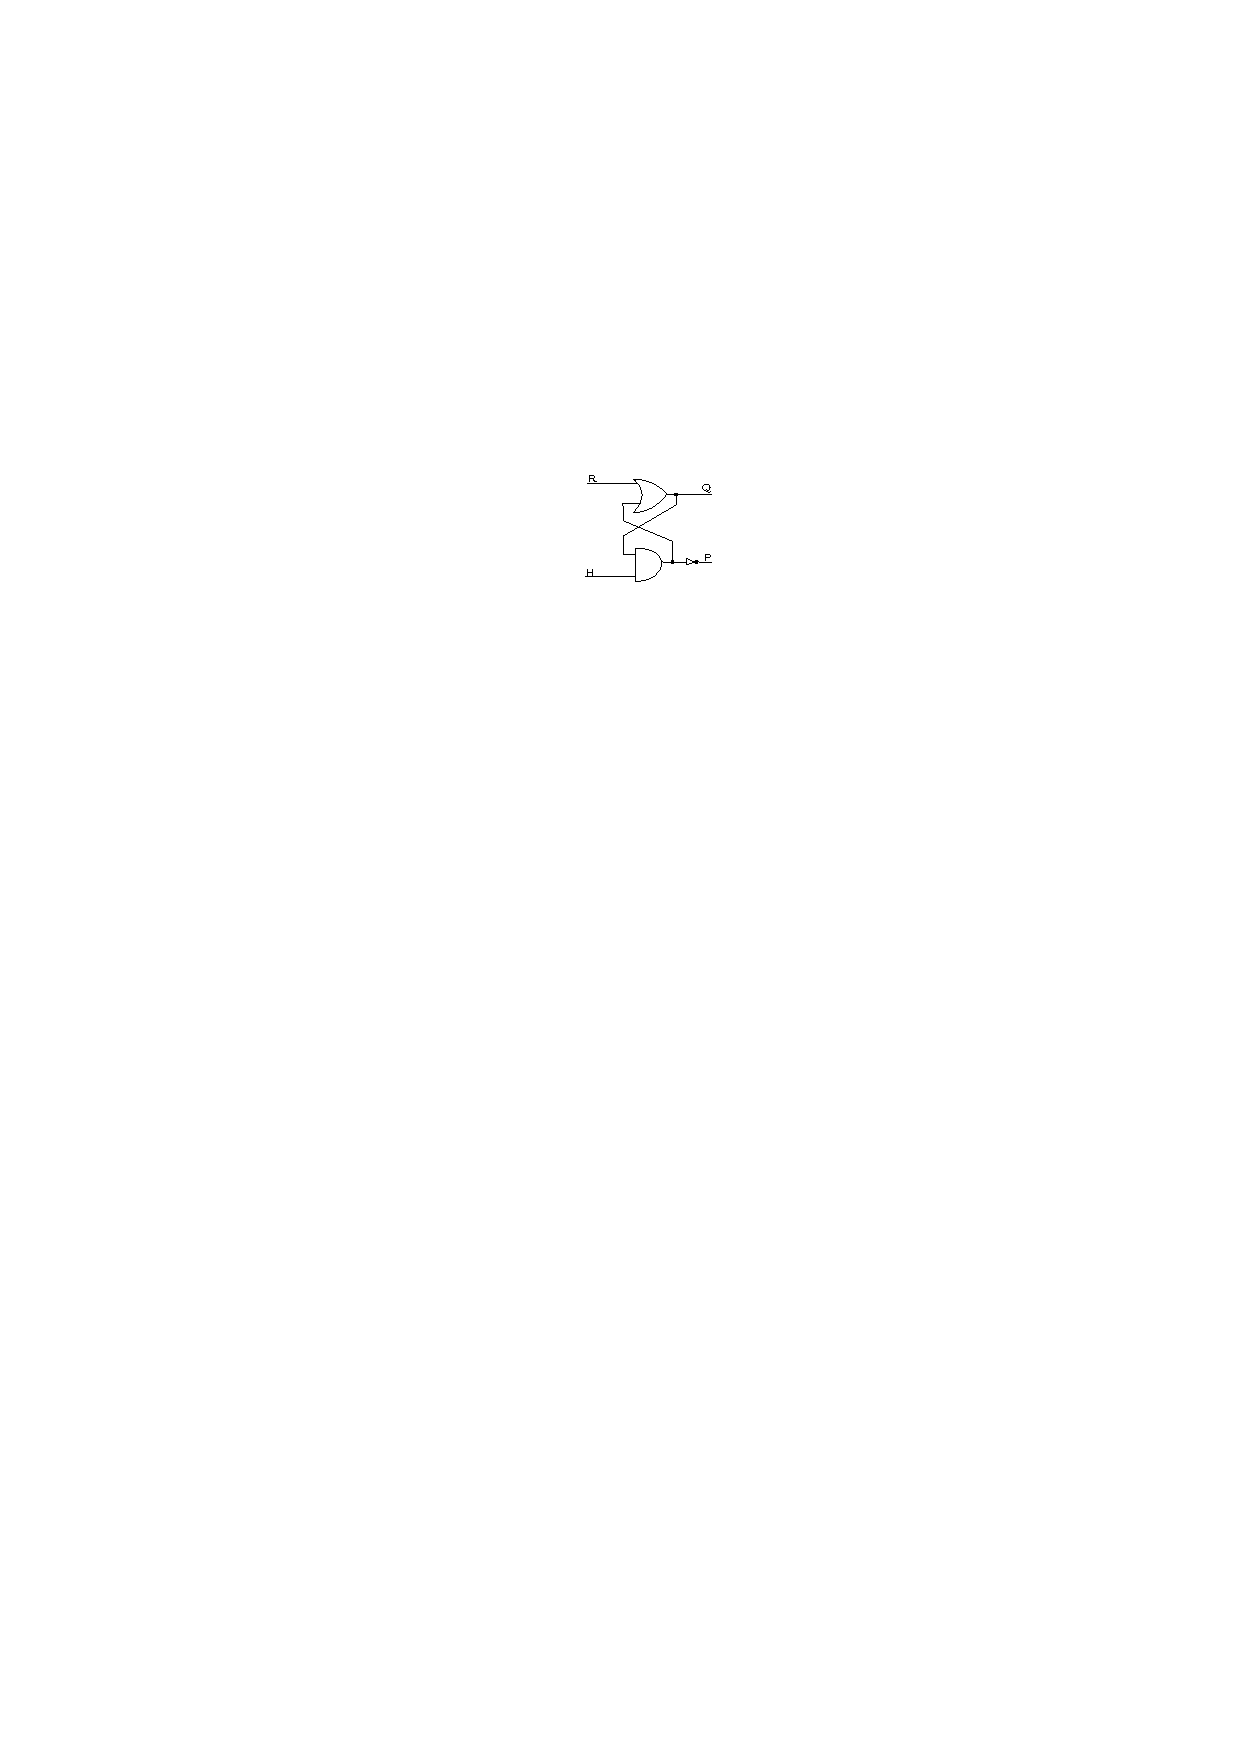
\includegraphics[width=0.3\textwidth]{fig/Q_basic1.pdf}
	\label{fig:Q_basic_1}
\end{figure}